\chapter{Atomic calculations with the effective charge model}
\addtocontents{toc}{\contentsline{chapter}{Atomic calculations with the effective charge model}{\protect\pageref{annotation}}}
\label{ch:Applications}

This chapter presents how the ECM can be used to calculate various atomic characteristics of atoms and ions. This includes global features, like binding energies and ionization cross-sections, as well as local ones, like electronic densities and scattering factors. The accuracy of the leading- and second-order ECM is investigated, as well as the appearance of key features, like the shell structure. The results obtained using the ECM are compared to ones coming from the TF and HF calculations in order to asses the practical usefulness of the ECM for atomic calculations.

\section{Ground state energies of neutral atoms}
\label{sec:ground-state-energ}

The first step in the ECM energy calculation is the choice of a particular electronic configuration, characterized by a set of occupied single-electron orbitals:~$|\lambda_1 ... \lambda_N \rangle$. We emphasize again, that the effective nuclear charge~$Z^*$ is identical for all single particle states in a given basis set, but we can choose different values of~$Z^*$ (and so different basis sets) for the description of different electronic configurations. The value of~$Z^*$ for each electronic configuration can be calculated according to
\begin{equation}
\Delta E^{(1)} (Z,Z^*) = \langle \lambda_1 \lambda_2 ... \lambda_n |
\widehat{W}^{(1)}(Z,Z^*)+\widehat{W}^{(2)}(Z^*) | \lambda_1 \lambda_2... \lambda_n \rangle = 0,
\end{equation}
which is required to obtain the value of the leading-order energy, as
\begin{equation}
E^{(0)} (Z,Z^*) = \langle \lambda_1 \lambda_2 ... \lambda_n |
\widehat{H}_0 | \lambda_1 \lambda_2... \lambda_n \rangle.
\end{equation}

For an illustrative example we investigated three different electronic configurations of the neutral cesium atom~$_{55}$Cs:~$[\mathrm{Xe}]6\mathrm{s}^{1}$,~$[\mathrm{Xe}]4\mathrm{f}^{1}$ and
$[\mathrm{Xe}]5\mathrm{d}^{1}$. The corresponding values of the effective charge were calculated as: $Z^*_{[\mathrm{Xe}]6\mathrm{s}^{1}} = 43.9986$, $Z^*_{[\mathrm{Xe}]4\mathrm{f}^{1}} = 43.8569$ and $Z^*_{[\mathrm{Xe}]5\mathrm{d}^{1}} = 43.9444$ giving the leading-order energies:~$E_{[\mathrm{Xe}]6\mathrm{s}^{1}} = -7361.18$, $E_{[\mathrm{Xe}]4\mathrm{f}^{1}} = -7346.19$ and $E_{[\mathrm{Xe}]5\mathrm{d}^{1}} = -7354.40$. Since the first one of these has the lowest energy, we expect it to correspond to the ground state and the other two to describe low-laying excited states. Indeed, the~$[\mathrm{Xe}]6\mathrm{s}^{1}$ configuration describes the ground state of~$_{55}$Cs in agreement with the so-called ``Aufbau'' principle or Madelung-Janet-Klechkovskii rule~\cite{Madelung1936,KlechkovskiiA1962justification, doi:10.1021/ed056p714}. The same is true for all atoms of the periodic table providing a simple and consistent choice of electronic configurations for any number of electrons. The fact that the extremely simple leading-order approximation is sufficient to describe correct fillings of atomic orbitals demonstrates a significant advantage of ECM over other single-parametric models such as the TFD or 1/Z-expansion.%Is it the case for~$1/Z?$. 

The values of total binding energies of the first 100 neutral atoms calculated with the ECM are compared to the values of highly accurate HF and DHF calculations on figure~\ref{ErrorComparisonFigure}. It can be readily seen that both the ECM and D-ECM lead to a uniform approximation i.e. with accuracy of:
\begin{equation} \label{Errorformula}
    \frac{E_{ECM}-E_{HF}}{E_{HF}} \approx 5\% - 6\%,
\end{equation}
independently of the number of electrons, already in the leading order. On the other hand, the~$1/Z$ expansion calculated up to first-order, only provides accuracy on the order of about~$12\%$. Furthermore, the inclusion of the single-electron second-order corrections to the ECM is enough to improve the accuracy to well below 1\%, as compared to the HF method, for all neutral atoms.

\begin{figure}
       \centering  
  \subfigure{\includegraphics[width=69mm]{Graphs/error_comparisonNoNR.pdf}}
  \subfigure{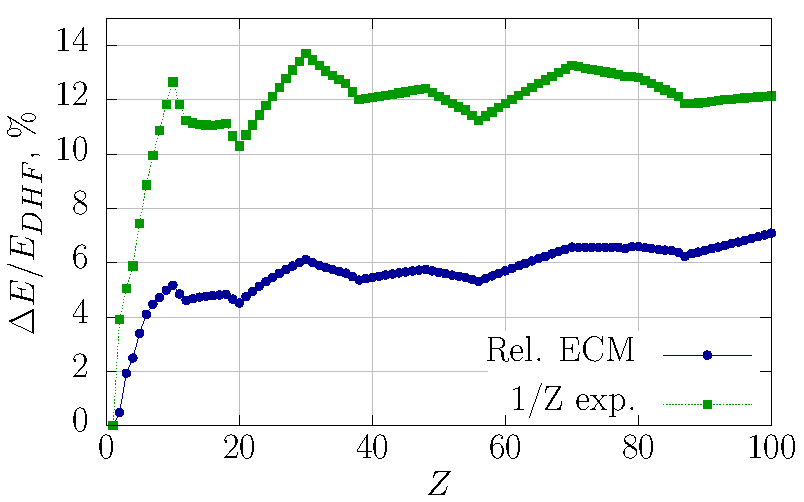
\includegraphics[width=69mm]{Graphs/Error_comparison.pdf}}
 \caption{Relative errors of the total binding energies calculated with the ECM as compared to the HF and DHF results~\eqref{Errorformula}. Left figure compares leading-order (blue) and single-electron second-order (green) ECM with the results of HF calculations~\cite{Saito2009836}. Right figure compares the leading-order D-ECM (blue) and first-order 1/Z expansion (green) to the results of DHF calculations~\cite{DESCLAUX1973311}. The corresponding numerical values of both non-relativistic and relativistic total binding energies are given in the Appendix~\ref{app:GroundStates}. This figure has been published as figure 1 in~\cite{Dzikowski_2021}.} \label{ErrorComparisonFigure}
\label{fig:my_label}
  \end{figure}

\begin{table}[b]%check values and add more digits to show differences
    \centering
    \begin{tabular}{cc|cccccc}
         Z &~$\rm{Element}$ &~$E^{(2)}_{\rm{single}}$ &~$E^{(2)}$ &~$\Delta E_{corr}$ &~$\rm{HF}$ &~$\rm{MCHF}$ & \rm{SDTQ}\\
         \hline
        \hline
         2 & He & -2.861 & -2.907 & 0.046 & -2.862 & -2.903 & 0.041 \\
         3 &Li & -7.411 & -7.462 & 0.051 & -7.433 & -7.477 & 0.044\\
         4 & Be & -14.52 & -14.69 & 0.165 & -14.57 & -14.67 & 0.093\\
         5 & B & -24.41 & -24.57 & 0.159 & -24.53 & -24.65 & 0.121\\
         6 & C & -37.49 & -37.64 & 0.148 & -37.69 & -37.84 & 0.150\\
         7 & N & -54.11 & -54.31 & 0.195 &-54.40 & -54.58 & 0.180\\
         8 & O & -74.38 & -74.65 & 0.268 & -74.81 & -75.05 & 0.245\\
         9 & F & -98.82 & -99.16 & 0.343 & -99.41 & -99.72 & 0.308\\
         \hline
    \end{tabular}
    \caption{Comparison of the second order single electron and double electron ground state energies with the single-configuration and multi-configuration numerical Hartree-Fock results.~$\Delta E_{corr}$ represent the electron-electron correlation energy calculated as the difference between the~$E^{(2)}_{\rm{single}}$ and~$E^{(2)}$, while SDTQ lists the corresponding Hartree-Fock result.}
    \label{tab:correlations}
\end{table}

This shows that the leading-order ECM and D-ECM give a particularly useful initial approximation to the orbitals of multi-electron atoms, and can be used a starting point for high-precision calculations, including those based on the HF method.

Following the considerations of section~\ref{sec:Green}, we can include electron-electron correlations, that is the double-electron second-order correction to the ECM. The resulting values of binding energy are in some cases already more accurate than the ones coming from the HF method and so have to be compared to the much more sophisticated MCFH procedure. Results for the first 10 neutral atoms are presented in table~\ref{tab:correlations}. Nevertheless, despite the promising accuracy of the second-order ECM, the largest source of uncertainty remains the neglect of higher orders of perturbation.

	\begin{figure} 
		\centering
		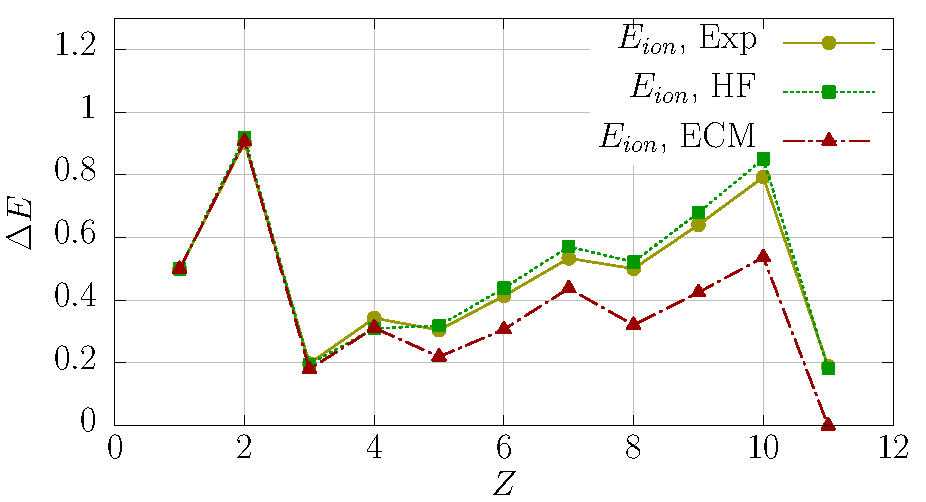
\includegraphics[width=120mm]{Graphs/Ionization.pdf} 
		\caption{Comparison of the first ionization energies of low-$Z$ neutral atoms, calculated with the full second-order ECM (red) with HF values~\cite{Saito2009836} (green) and experimental values from the NIST database~\cite{NIST} (yellow).} \label{Ionization}
		 		\end{figure}
	
	\begin{table}[b]%check values and add more digits to show differences
    \centering
    \begin{tabular}{cc|ccc}
         Z &~$\rm{Element}$ &~$\Delta E^{(2)}_{\rm{aff}}$ &~$\Delta E^{\rm{DFT}}_{\rm{aff}}$ &~$\Delta E^{\rm{exp}}_{\rm{aff}}$ \\
        \hline
        \hline
         1 & H & 0.87 & 0.84 & 0.75 \\
         2 & He & -1.27 & 0.03 & - \\
         3 & Li & 0.89 & 0.50 & 0.62 \\
         4 & Be & -4.23 & 0.03 & - \\
         5 & B & -4.30 & 0.43 & 0.28 \\
         6 & C & -2.81 & 1.39 & 1.26 \\
         7 & N & -6.64 & 0.23 & - \\
         8 & O & -6.19 & 1.83 & 1.46 \\
         9 & F & -5.3 & 3.74 & 3.40 \\
         \hline
    \end{tabular}
    \caption{Comparison of electron affinities of neutral atoms, between the full second-order ECM, DFT calculations~\cite{DFTaffinities}, and experimental measurements.} %[ref.].}
    \label{tab:Affinities}
\end{table}

\section{Ionization energies}

Since the number of electrons and the full nuclear charge~$Z$ are independent parameters in the ECM, it can also be used for the description of ions. By fixing~$Z$ and calculating the effective charge~$Z^*$ for electronic configurations with different numbers of electrons, we can describe positively-charged ions and find corresponding ionization energies. The first ionization energies for all atoms up to magnesium have been plotted in figure~\ref{Ionization}. The comparison to the HF calculation and experimental values shows that the relative error is larger than for energies themselves (as should be expected, since the errors have the same magnitude while values are much smaller), but the shape and general features of the ionization curve are well represented. This is not the case for other analytical approximations such as the TF model.

	Furthermore, by setting the full nuclear charge smaller than the number of electrons we can also investigate negative ions and their ionization energies, often referred to as electron affinities. This is a particularly interesting test of any computation scheme, as the extra electron of a negative ion is bound primarily by electron-electron correlation rather than the Coulomb force. Electron affinities of the first nine neutral atoms are presented in table~\ref{tab:Affinities}.
	
\begin{figure*}
  \centering  
  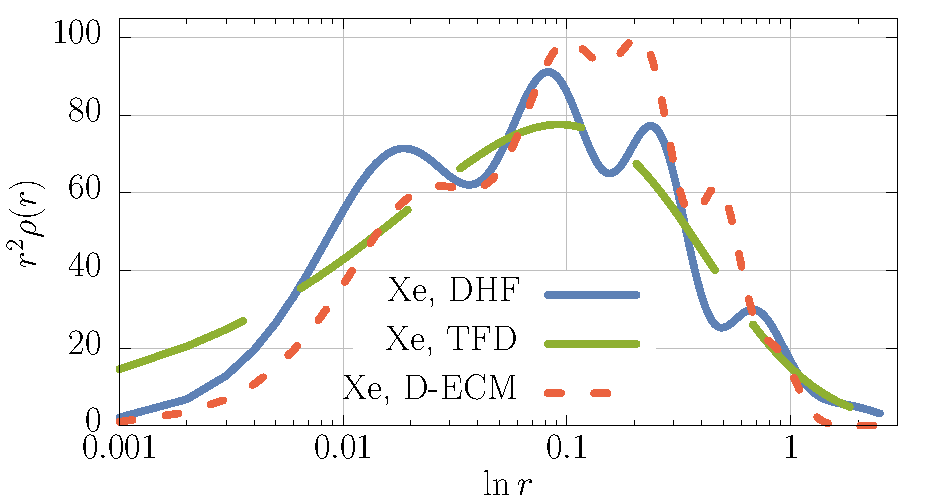
\includegraphics[height=37mm]{Graphs/xe_rel_rho.pdf}
 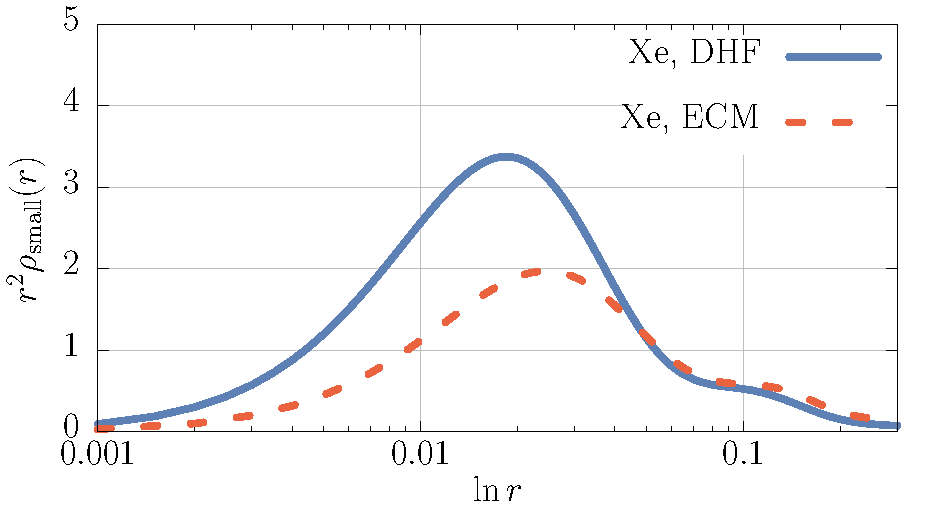
\includegraphics[height=37mm]{Graphs/xe_rel_rho_small.pdf}
  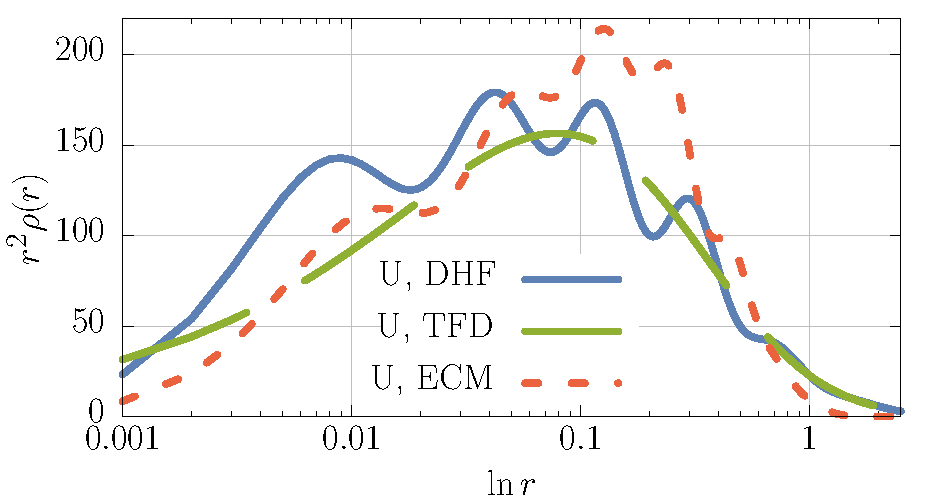
\includegraphics[height=37mm]{Graphs/u_rel_rho.pdf}
  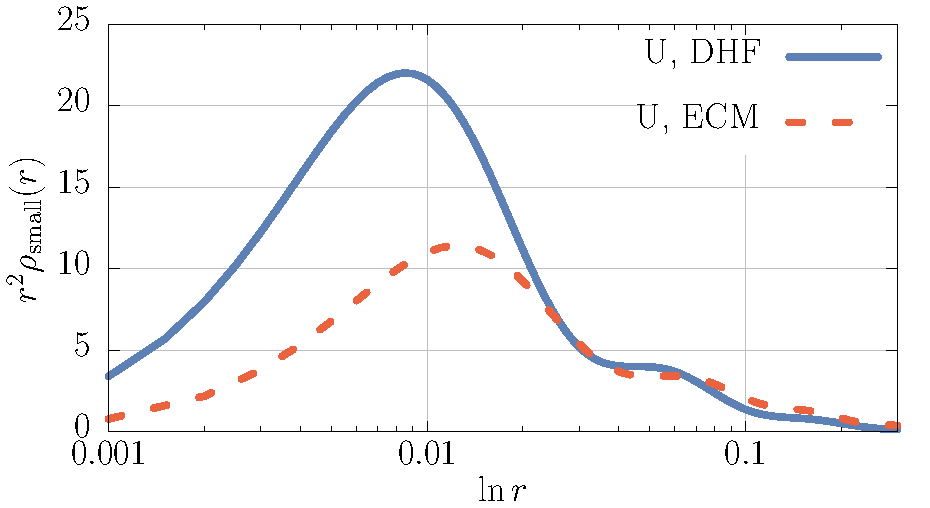
\includegraphics[height=37mm]{Graphs/u_rel_rho_small.pdf}
  \caption{Total radial electronic densities (left)
    and densities composed from the small components of the
    Dirac wave functions (right) of neutral
    xenon $_{54}$Xe (top) and neutral uranium
    $_{92}$U (bottom). Dashed, red line is the
    leading-order effective charge approximation, blue line
     represents the results of the numerical
    solution of DHF (obtained via GRASP2k~\cite{jonsson_new_2013,
      DYALL1989425}) and  green, long-dashed line stands for the TFD model. This figure has been published as figure 2 in~\cite{Dzikowski_2021}.}
  \label{Rel_rhoPlot}
\end{figure*}

\section{Electron densities}

In this section we demonstrate that the presented approach is suitable to provide useful approximations not only to the integral characteristics of the atom, but also to local ones, by investigating the ECM approximation to electron densities.

\subsection{Zeroth-order densities}

In the secondary-quantized representation, the density operator is given by
\begin{equation}
    \widehat{\rho}(r)=\sum_{\lambda,\lambda'}\psi_{\lambda}^\dag(r)\psi_{\lambda'}(r) \widehat{a}_{\lambda}^\dag \widehat{a}_{\lambda'}.
\end{equation}
Taking the expectation value of~$\widehat{\rho}$ with the leading-order wavefunctions of the ECM we get the leading order density
\begin{equation} \label{densityFormula}
    \langle\Psi^{(0)}|\widehat{\rho}(r)|\Psi^{(0)}\rangle = \sum_k \langle \lambda_k| \vec{r}\rangle \langle \vec{r}|\lambda_k \rangle,
\end{equation}
as a a sum of squares of hydrogen-like bound states. This means that the leading-order density is given by a simple combination of exponentials and polynomials,
allowing its use in numerical plasma~\cite{chung_flychk:_2005} or
description of ionization in particle-in-cell (PIC) computer codes
for laser-matter interactions~\cite{Arber_2015}. Furthermore, since the ECM, unlike the DHF and TF calculations, provides fully analytical expressions for electronic
densities and is therefore particularly useful for applications
requiring repeated calculations. Relatively simple expressions
resulting from our model can be incorporated into existing
software, used in the description of X-ray scattering on M\"{o}ssbauer
crystals~\cite{Sturhahn2000}. Explicit expressions are provided in Appendix~\ref{app:zeroDensities}.

In figure~\ref{Rel_rhoPlot} we plot the resulting
dependence of electronic densities on the radial coordinate~$r$ for
selected neutral atoms. Despite the fact that the effective charge
model underestimates the density for high~$r$, it agrees well with the
DHF result already in the leading-order
approximation. Contrary to the TFD model, it correctly
reproduces all of the qualitative features, including all density
oscillations and the overall asymptotic behavior. In addition, we
point out that the TFD model, unlike the
non-relativistic TF, does not have a
universal dependence on the charge of the nucleus~\cite{qua.560200311}. For this reason, in
order to obtain the electronic density, the TFD equation
needs to be repeatedly solved numerically, which is a nontrivial
procedure.

		\begin{figure} 
 			\centering
 			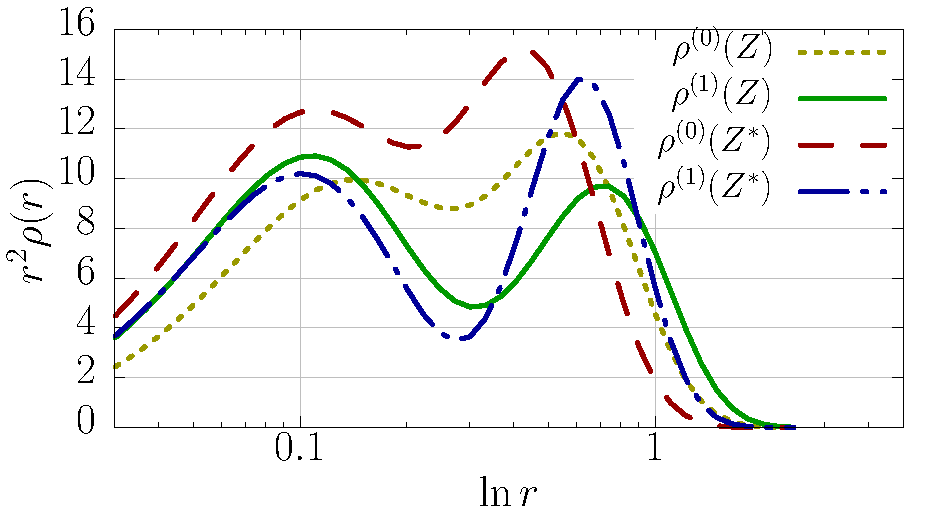
\includegraphics[width=69mm]{Graphs/Ne_rho.pdf} 
 			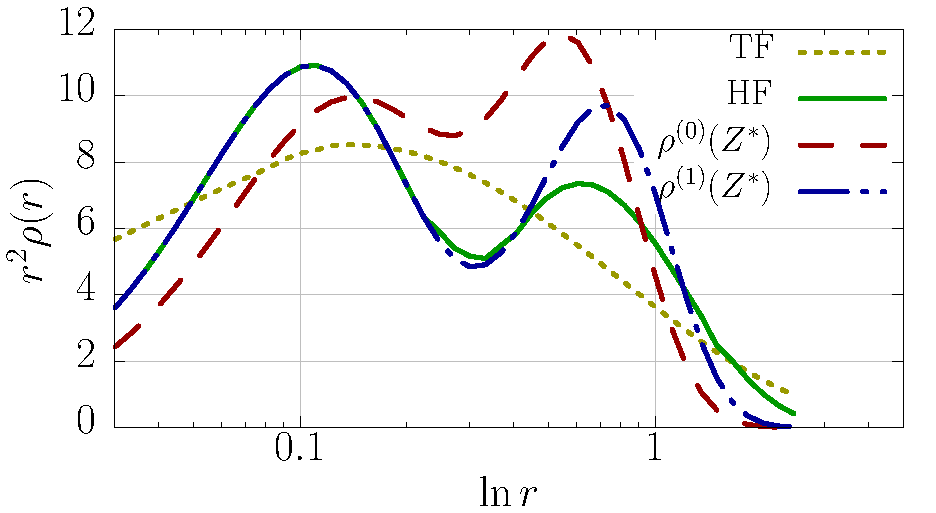
\includegraphics[width=69mm]{Graphs/Ne_rho2.pdf} 
 			\caption{Comparison of electron density of neutral neon using the zeroth-order and first-order ECM, with the zeroth-order and first order~$1/Z$ expansion (left), as well as with the HF results~\cite{jonsson_new_2013} and the TF model~\cite{LandauQM} (right). Red and blue are the zeroth- and first-order ECM calculations respectively. Yellow and green represent either the~$1/Z$ expansion (left) or the TF and HF results (right).} \label{NeonPlot}
 		\end{figure}

\subsection{First-order densities}

Using the the same approach as for energies, we can also easily derive analytical expressions for the first-order electron densities. Let's recall the perturbative expansion due to the operator~$W$ of our
multi-electron wave function
\begin{equation}
|\Psi \rangle = |\Psi^{(0)} \rangle + |\Psi^{(1)}\rangle +... = |\Psi^{(0)} \rangle + \sum_{\sigma} |\sigma\rangle \frac{\langle \sigma|\widehat{W}| \Psi^{(0)} \rangle}{E_0 - E_\sigma} +...~~,
\end{equation}
and split the intermediate states into single-electron and double-electron contributions just like in the calculation of energies
\begin{equation}
|\Psi \rangle = |\Psi^{(0)} \rangle + |\Psi^{(1)}_{\rm{single}}\rangle + |\Psi^{(1)}_{\rm{double}}\rangle...~~.
\end{equation}

Since~$\widehat{\rho}(r)$ it is a single-particle operator, only the single-electron part of~$\Psi^{(1)}$ will contribute to its expectation value, so that we have
\begin{align}\label{FirstDensityEq}
\widehat{\rho}(r)_{\Psi}^{(1)}&=\langle\Psi^{(0)}+\Psi^{(1)}_{\mathrm{single}}|\widehat{\rho}(r)|\Psi^{(0)}+\Psi^{(1)}_{\mathrm{single}}\rangle \nonumber
\\
&=\langle\Psi^{(0)}|\widehat{\rho}(r)|\Psi^{(0)}\rangle + 2\langle\Psi^{(0)}|\widehat{\rho}(r)|\Psi^{(1)}_{\mathrm{single}}\rangle + \langle\Psi^{(1)}_{\mathrm{single}}|\widehat{\rho}(r)|\Psi^{(1)}_{\mathrm{single}}\rangle \nonumber
\\
&= \sum_k \langle \lambda_k| \vec{r}\rangle \langle \vec{r}|\lambda_k \rangle + 2\sum_{l,k} \langle \lambda_k(r) | \Psi^{(1)}_{\mathrm{single},\lambda_l}(r) \rangle .
\end{align} 

Just as for energies, we can make use of the RCGF, to get the explicit expression for the first order wave function, as
\begin{equation} \label{1wave}
|\Psi^{(1)}_{\mathrm{single}}\rangle &= \sum_k |\Psi^{(1)}_{\mathrm{single},\lambda_k} \rangle = \sum_k \widetilde{G}_{\lambda_k} \widehat{W}^{(1)} |\lambda_k \rangle + \sum_{k,l \neq k} \widetilde{G}_{\lambda_k} \langle \lambda_l |\widehat{W}^{(2)}| \lambda_k \lambda_l \rangle,
\end{equation}
with implied exchange integrals.

\begin{figure*}
  \centering  
  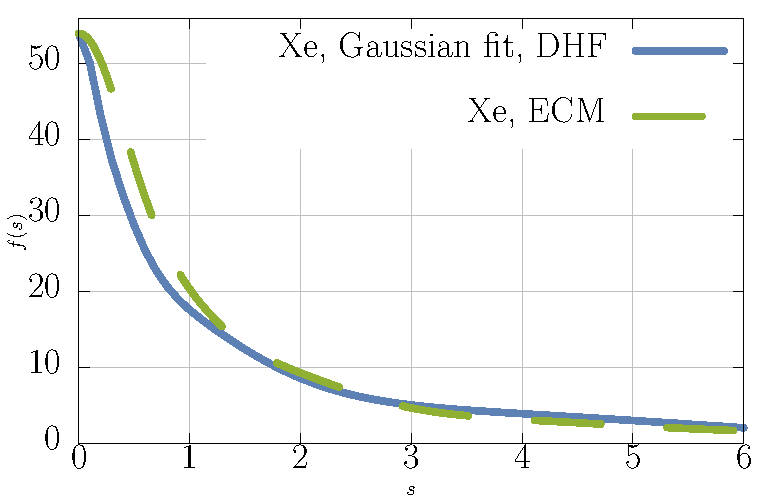
\includegraphics[width=69mm]{Graphs/asf_Xe.pdf}
  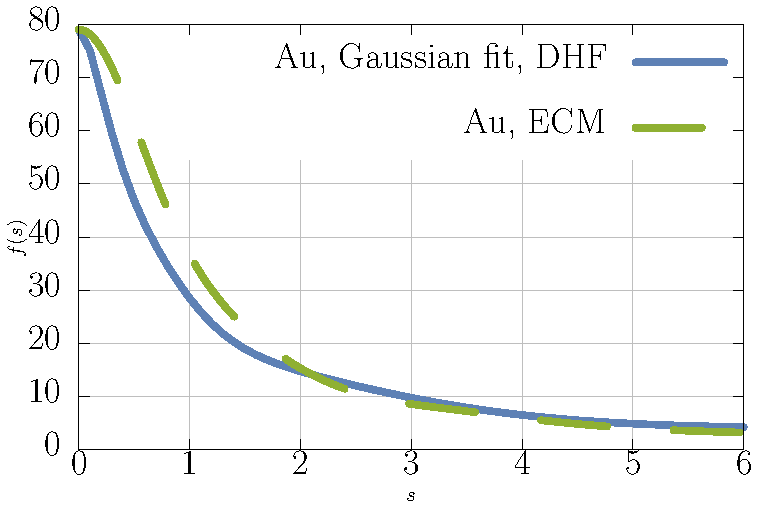
\includegraphics[width=69mm]{Graphs/asf_Au.pdf}
  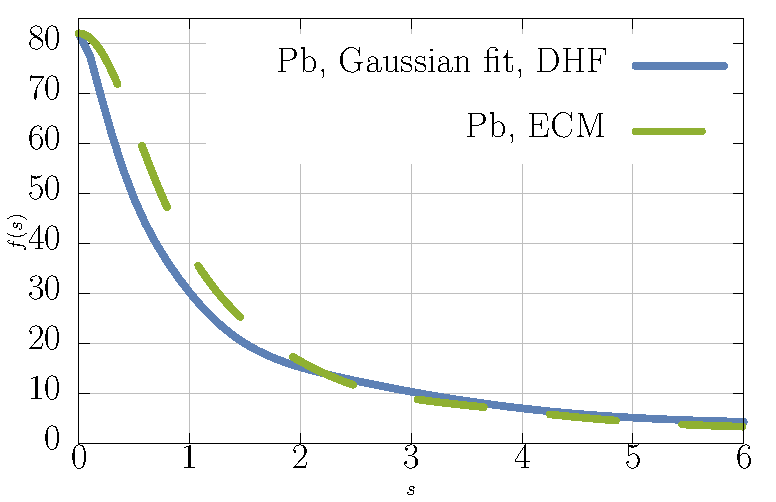
\includegraphics[width=69mm]{Graphs/asf_Pb.pdf}
  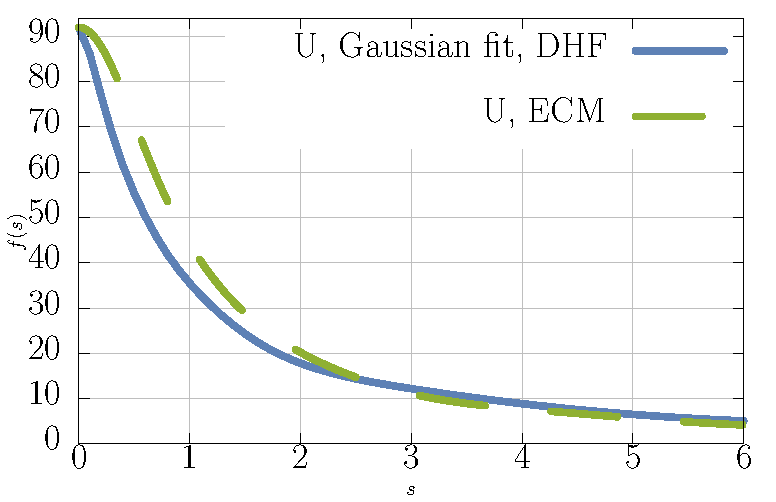
\includegraphics[width=69mm]{Graphs/asf_U.pdf}
  \caption{Atomic scattering factors of neutral xenon
   ~$_{54}$Xe, gold~$_{79}$Au, lead
   ~$_{82}$Pb and uranium~$_{92}$U atoms, as a
    function of the scattering parameter
   ~$s = \sin\theta / \lambda,\ [\textup{\AA}^{-1}]$, with~$\theta$
    being Bragg's angle. The quantity~$s$ is related to the absolute
    value of~$q$ from Eq.~(\ref{eq:15}) as
   ~$q = 4\pi s \cdot 0.529177$. Dashed, green line is the analytic
    result via Eq.~(\ref{eq:15}) of the ECM, while the solid
    blue curve is a Gaussian fit of DHF from
   ~\cite{DHFscatter}. This figure has been published as figure 4 in~\cite{Dzikowski_2021}.}
  \label{fig:ASF}
\end{figure*}

As an example, we have plotted the radial dependence of the electronic density of the neutral neon atom in figure~\ref{NeonPlot}. The left plot compares the ECM with the~$1/Z$ expansion (wchich corresponds to setting~$Z=Z^*$). We can see that the difference between them is significant and that the effective charge adjusts the width and height of the density plot. However, it also shows, that the relative height of subsequent density maxima can only be obtained with first order corrections. The right plot meanwhile compares the ECM to the results of HF and TF calculations. It is clear that unlike the TF model, the ECM reproduces the full shell structure with correct number of density maxima already in the zeroth-order. Furthermore, the first-order density aligns very well with the results of the HF calculation, except for large radial distances, where the ECM slightly underestimates the decay rate.

It is instructive to consider, how each of the terms in~\eqref{FirstDensityEq} scales with the effective nuclear charge, to see that subsequent terms do indeed get smaller rather quickly, ensuring fast convergence of the perturbation series. As explained in chapter~\ref{ch:ECM}, the charge/scale invariance of the Schr\"{o}dinger equation leads to simple scaling of wavefunctions and potentials:
\begin{align}
    \Psi_{\lambda}(r) \propto (Z^*)^\frac{3}{2},~~~~~~~~~~~~G(x,y) \propto Z^*,~~~~~~~~~~~~W_{k,\lambda,\lambda} \propto Z^*.
\end{align}
This in tern translates to scaling of density elements containing~$\widehat{W}^{(2)}$, as
\begin{equation}
\langle\Psi^{(0)}|\widehat{\rho}(r)|\Psi^{(0)}\rangle \propto (Z^*)^3 ,
\end{equation} 
\begin{equation}
\langle\Psi^{(0)}|\widehat{\rho}(r)|\Psi^{(1)}\rangle \propto (Z^*)^2 ,
\end{equation} 
\begin{equation}
 \langle\Psi^{(1)}|\widehat{\rho}(r)|\Psi^{(1)}\rangle \propto Z^* .
\end{equation} 
Elements containing~$\widehat{W}^{(1)}$ scale in the same way, with an extra factor of~$(Z-Z^*)$.

\section{Atomic scattering factors}
\label{sec:atom-scatt-fact}

Another example of a useful observable characteristic that can be easily approximated using the ECM, are the atomic scattering factors. They
are usually expressed~\cite{hau2012high} as the Fourier transforms of electronic density
\begin{align}
  f(\vec{q}) = \int \rho(\vec{r})e^{i \vec{q} \cdot \vec{r}}
  d\vec{r}, \label{eq:15}
\end{align}
which in the leading-order can be easily be calculated analytically (see
Appendix~\ref{app:scatter} for further details).

The atomic scattering factors are very important for crystallography
and X-ray physics, since the crystal polarizability~$\chi$ as the
function of X-ray frequency~$\omega_{\mathrm{r}}$, can be evaluated by
employing the following relation~\cite{ahmadi_feranchuk_2013}
\begin{align}
  \chi(\vec g, \omega_{\mathrm{r}}) = \frac{4 \pi S(\vec g)}{\Omega_{0}
  \omega_{\mathrm{r}}^{2}}
 f(\vec g), \label{eq:17}
\end{align}
where~$\Omega_0$ is the volume of a crystal cell,~$\vec g$ the
reciprocal lattice vector and~$S(\vec g)$ the structure factor of the
crystal.

In figure~\ref{fig:ASF} we present the results for neutral
xenon~$_{54}$Xe, gold~$_{79}$Au, lead~$_{82}$Pb and uranium~$_{92}$U
atoms. Our analytical expressions for atomic scattering factors are
comparable to the DHF calculation to within~$25\%$. At the same time, they are much more convenient to work with, being composed of finite sums of elementary functions rather than Gaussian fits to specific pre-calculated points.

\section{Highly charged ions}
\label{sec:highly-charged-ions}

In recent years there has been particular interest~\cite{IonsInterest} in the study both theoretical~\cite{IonsTheory} and experimental~\cite{IonsExperiment} of highly charged ions (HCI). Applications have been found in many different areas of modern physics, from optical clocks~\cite{IonsClocks} to fundamental physics~\cite{IOnsFundamental}. Since higher orders of the ECM are proportional to decreasing powers of~$Z$ and~$Z^*$, it naturally becomes more accurate in describing HCI, as compared to neutral atoms.

The results of the calculation of leading-order electronic densities of HCI are presented
in figure~\ref{fig:HCI}. The electronic densities calculated using the ECM, despite being
very simple analytical expressions,
coincide remarkably well with the ones obtained from numerical
solutions of the DHF equations.

\begin{figure*}
  \centering  
  \subfigure{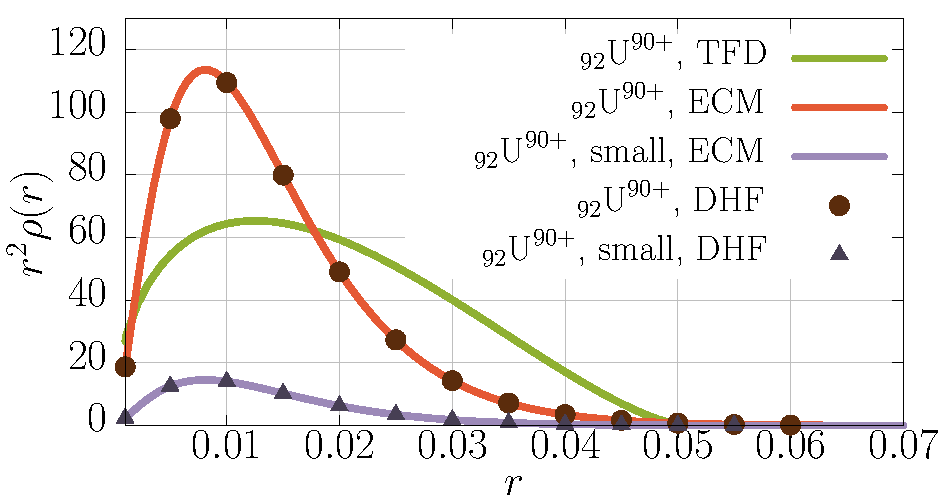
\includegraphics[width=69mm]{Graphs/helu_rel_rho.pdf}}
  \subfigure{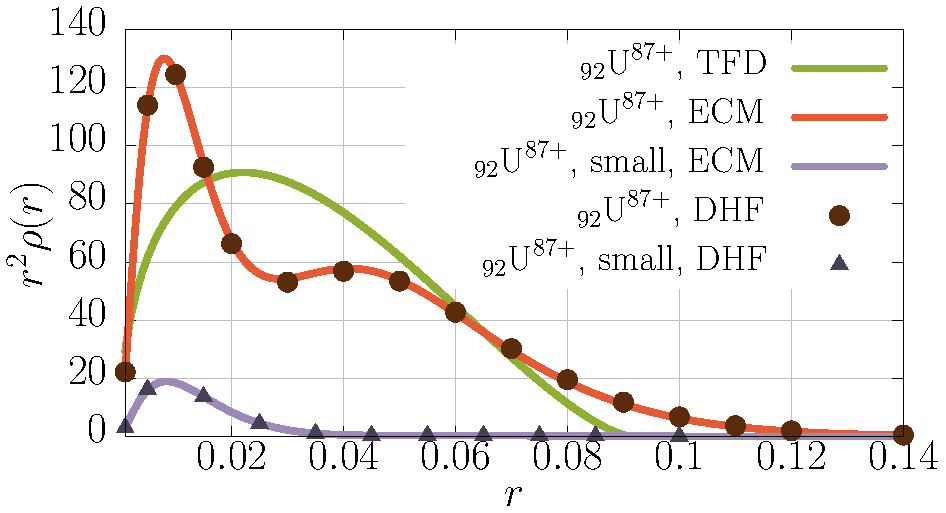
\includegraphics[width=69mm]{Graphs/blu_rel_rho.pdf}}
  \caption{Total and small component electronic
    densities of highly charged uranium \changeR{$_{92}$U$^{90+}$ and
     ~$_{92}$U$^{87+}$}. \changeR{Red (total) and purple (small)} lines are the \changeR{leading-order}
  ECM \changesR{densities},  \changeR{black circles (total) and black triangles (small) represent} results of the DHF \changeR{densities} (obtained via GRASP2k
   ~\cite{jonsson_new_2013, DYALL1989425}),  and the solid green stands for TFD model. This figure has been published as figure 3 in~\cite{Dzikowski_2021}.}
  \label{fig:HCI}
\end{figure*}

\section{Photoionization cross-section}
\label{sec:photo-ionis-cross}	

As one more practical application of the ECM, we
present the calculation of the total cross section for the
photoionization of a multi-electron atom. From first principles it can
be shown~\cite{PhysRev.134.A898}, that within the dipole approximation,
the differential cross-section for a photon with momentum~$k$ to
overcome an ionization energy~$E_0$ and produce an outgoing electron
with momentum~$p$ can be calculated according to
\cite{mikhailov1969relativistic}
\begin{equation}\label{PICformula}
  \frac{d \sigma}{d \Omega} = \frac{\alpha p (k+E_0)}{2 \pi k}
  \left|\int \psi^{\dagger}_f(\vec
    r)\vec{\alpha}\psi_i(\vec r) d\vec{r}\right|^2,
\end{equation}
where~$\psi_i$ is the initial bound-state wave function and the final
wave function can be described, as
\begin{equation}
  \psi_f(\vec r) = 4\pi \sum_{\kappa',m'}
  \xi_{\kappa',m'}\left(\frac{\vec{p}}{p}\right)e^{-i
    \delta_{\kappa'}}\psi_{\rm free}(\vec r),
\end{equation}
where~$\xi$ are normalized spinors~\cite{lifshitz1974relativistic},
describing the angular distribution and polarization of the outgoing
electrons, and~$\delta_{\kappa'}$ are phase shifts, ensuring outgoing
solutions.

Within the ECM,~$\psi_i$ and~$\psi_{\rm{free}}$ are
described by negative and positive-energy solutions to the Dirac
equation for hydrogen with relevant effective charge. Summing over all
electrons in a given atom or ion allows us then to analytically
calculate the total effective cross-section for the photoionization
process within the leading-order ECM (see Appendix~\ref{app:photo} for details).

In the presented calculation both initial and final wave functions have
been described using the same value of effective charge, so that they correspond to the same
effective potential. It is possible because the total cross-section
includes the summation over a full set of intermediate electron
excitations. The same approximation was employed in~\cite{YEH19851}.  On the other hand, the ionization
energies~$E_k$ are calculated separately for each electron, by finding
the "valence effective charge"~$Z^*_k$, defined by requiring the first
order correction to~$E_k$ to vanish. Hence it can be found by solving
\begin{equation}
  \Delta E^{(1)}_{\lambda_0}(Z^*_k)-\Delta E^{(1)}_{\lambda_k}(Z^*_k)=0,
\end{equation}
where~$\lambda_0$ is the ground state configuration and~$\lambda_k$
the final configuration, i.~e. without the ionised electron.
Figure~\ref{fig:PIC} presents the comparison of the results for two
example atoms with the analogous non-relativistic calculation, as well
as results of the Hartree-Fock-Slater (HFS) calculations~\cite{YEH19851}. It can be seen that shifting to a relativistic
description improves the accuracy of such calculation. The results
show that the ECM gives reasonable qualitative
description and can be used for approximating physical characteristics
dependent on transition matrix elements.

\begin{figure*}
	\centering  
	\subfigure{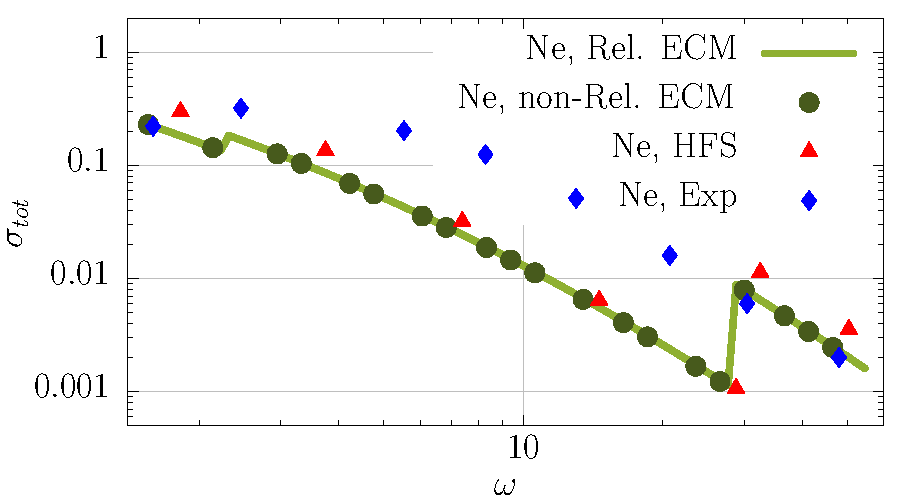
\includegraphics[width=69mm]{Graphs/photo_neon.pdf}}
	\subfigure{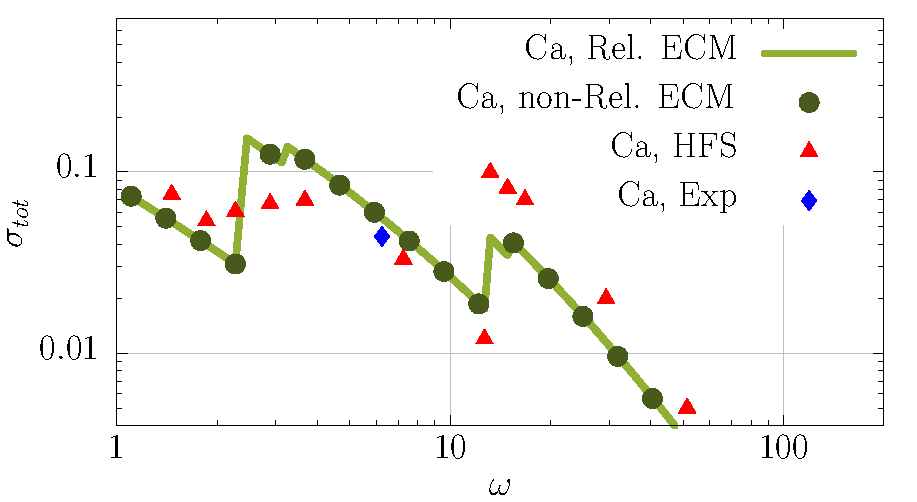
\includegraphics[width=69mm]{Graphs/photo_calcium.pdf}}
	\caption{Comparison of the ECM (circles)
		and D-ECM (solid) calculation of the total
		photoionization cross-section for neon~$_{10}$Ne (left)
			and calcium~$_{20}$Ca (right). Hartree-Fock-Slater calculation
		results are marked with red triangles and taken from~\cite{YEH19851}.Experimental data are taken
			from~\cite{MARR1976497} for neon and from~\cite{L_rch_1999} for calcium. This figure has been published as figure 5 in~\cite{Dzikowski_2021}.}
	\label{fig:PIC}
\end{figure*}

\section{Transition probabilities}
\label{sec:TP}

Transitions between electronic states are observed as emission lines in the spectrum of a given atom or molecule. The observed intensity is related to the probability of the transition, which is usually expressed per unit time ($\rm{sec}^{-1}$). For the purposes of theoretical analysis it is more convenient to analyse atomic transitions in terms of corresponding dimensionless quantities called oscillator strengths, which can be defined mathematically, as~\cite{OscillatorsDefinition}
\begin{equation}
    f = \frac{1}{8 \pi^2} g \lambda A^2,
\end{equation}
where~$g$ is the ratio of statistical weights of the involved atomic states,~$\lambda$ the corresponding wavelength and~$A$ the Einstein coefficient~\cite{EinsteinCoeff}.

The corresponding cross-section is then given by~\cite{EinsteinCoeff}
\begin{equation}
\sigma = \frac{\alpha \pi}{2} f \phi_{\omega},
\end{equation}
where~$\phi_{\omega}$ is the normalized angular frequency distribution \footnote{Even though oscillator strengths are defined so as to represent the normalized probability of transition, they can in some special cases be larger that unity~\cite{HENS2008391}.}.

\subsection{Non-relativistic calculation of transition probabilities}
	
	Using the Schr\"{o}dinger Hamiltonian, the oscillator strength of E1 transitions in the dipole representation between states described by the wavefunctions~$\psi_i$ and~$\psi_f$ can be calculated according to~\cite{demtroder2002laser}
\begin{equation}
    f = 2(E_f-E_i) \left|\langle \psi_i|\vec{r}|\psi_f \rangle \right|^2,
\end{equation}
where~$\vec{r}$ is a vector of all of the spatial coordinates involved (and so dimension~$3N$).

Within the leading-order ECM, we have:
\begin{align}
    &\Delta E (Z^*) \sim (Z^*)^2 \Delta E\\
    &\psi(r) \sim (Z^*)^{3/2}\psi(Z^* r),
\end{align}
which makes the leading order oscillator strengths independent of effective charge
\begin{equation}
    f^{(0)} \sim (Z^*)^0,
\end{equation}
and by extension independent of the total charge~$Z$. For these reason ECM can only be used to approximate oscillator strengths when higher orders are included. The first order correction to the wavefunctions is given by
\begin{equation}
    \psi^{(1)}(r) = \psi_0 W \widetilde{G}_{\psi_0},
\end{equation}
where the Greens function sums over all virtual states differing from~$\psi^{(0)}$ by at most two electrons. However since~$\vec{r}$ is a single-electron operator, only states that differ by one electron from either~$\psi_i$ or~$\psi_f$ will contribute in the first order. That is, for a transition
\begin{equation}
    |\lambda_1 ... \lambda_{n-1}, \lambda \rangle \rightarrow |\lambda_1 ... \lambda_n,\chi \rangle,
\end{equation}
the first order correction to~$\langle \psi_i^{(0)}|\vec{r}|\psi_f^{(0)} \rangle$ is given in its entirety by:
\begin{align}
   \Delta f^{(1)} =& \sum_i \langle \lambda \lambda_i|\widehat{W}|\lambda_i \rangle \widetilde{G}_{\lambda} \vec{r} | \chi \rangle +\langle \chi \lambda_i|\widehat{W}|\lambda_i \rangle \widetilde{G}_{\chi} \vec{r} | \lambda \rangle \nonumber
   \\
   &+ \sum_{i,j} \langle \lambda \lambda_i|\widehat{W}|\chi \rangle \widetilde{G}_{\lambda_i} \vec{r} | \lambda_j \rangle  + \langle \chi \lambda_i|\widehat{W}|\lambda \rangle \widetilde{G}_{\lambda_i} \vec{r} | \lambda_j \rangle 
\end{align}
with implied anti-symmetric exchange.

Corresponding results of the oscillator strengths for the two primary transitions in the low-$Z$ helium-like ions, namely~$1s^2 \rightarrow (1s2p)^1P_1$ and~$1s^2 \rightarrow (1s3p)^1P_1$ are presented in figure~\ref{OscillatorPlot}. We can see that the dependence on nuclear charge, absent from the zeroth-order result, is correctly reproduced in first order, with the accuracy improving with increasing charge.

\begin{figure}
    \centering
    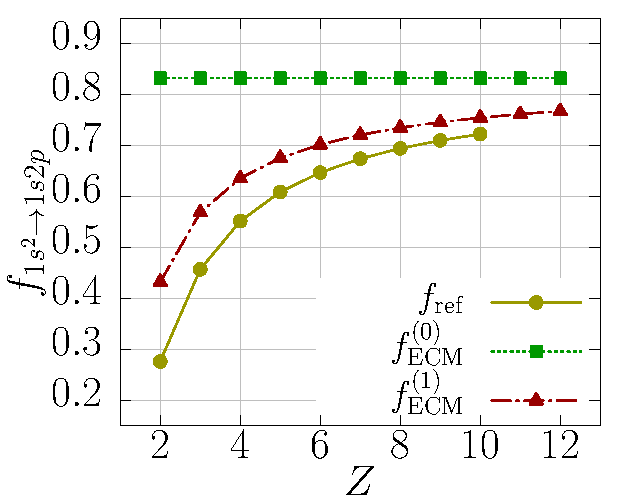
\includegraphics[width=69mm]{Graphs/OscillatorHe1s2p.pdf}
    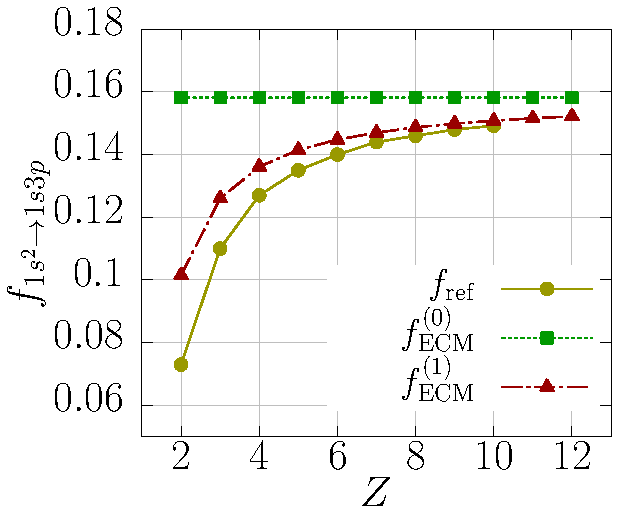
\includegraphics[width=69mm]{Graphs/OscillatorHe1s3p.pdf}
    \caption{Comparison of the zeroth-order (green) and first-order (red) oscillator strengths for the~$1s^2\rightarrow 1s2p$ (left) and~$1s^2\rightarrow 1s3p$ (right) transitions in helium-like ions with the corresponding reference values from the NIST database~\cite{NIST}.}
    \label{OscillatorPlot}
\end{figure}

\subsection{Gauge invariance of matrix elements}

Oscillator strengths can be expressed in terms of position matrix elements as~\cite{demtroder2002laser}
\begin{equation}
f_{i \rightarrow j} = \frac{2}{3} \frac{\Delta E_{ij}}{g_i} |\langle \psi_i|\vec{r}|\psi_j \rangle|^2 ,
\end{equation}
or in terms of momentum matrix elements as
\begin{equation}
f_{i \rightarrow j} = \frac{2}{3} \frac{1}{g_i \Delta E_{ij}} |\langle \psi_i|\vec{p}|\psi_j \rangle|^2 ,
\end{equation}
where~$\Delta E_{ij}$ is the energy difference between the two states between which the transition occurs, and~$g_i$ is the statistical weight of the state~$i$.

In principle, the two formulas above should be consistent (that is produce the same~$f$), however this is often not the case for many calculation schemes, because of incompatible numerical approximations. In fact, the equation obtained by equating the above two
\begin{equation} \label{consistency}
|\langle \psi_i|\vec{p}|\psi_j \rangle| = \Delta E_{i j} |\langle \psi_i|\vec{r}|\psi_j \rangle|,
\end{equation}
is sometimes used as an accuracy check of the approach used. In our case, it is trivially satisfied in the zeroth order, since by ground rules of quantum mechanics we always have
\begin{equation}
\widehat{p} = i [\widehat{H}_0,\widehat{r}] = i (\widehat{H}_0 \widehat{r} - \widehat{r} \widehat{H}_0),
\end{equation}
and if we multiply this relation by~$| \lambda \rangle$ states on both sides (which are exact eigenfunctions of~$\widehat{H}_0$), we immediately get (\ref{consistency}). The question of whether it is satisfied in the full second order energy calculation is less obvious, but can relatively easily be verified numerically.

\subsection{Relativistic calculation of transition probabilities}

For high-$Z$ atoms and ions the relativistic corrections to transition probabilities become important. An even more pronounced feature of the Dirac theory is that many of the non-relativistically forbidden transitions become possible. In particular, the so-called magnetic transitions, that is those where the multipole of the photon field causing the transition is not equal to the change in the angular momentum quantum number. The full relativistic calculation is somewhat more involved due to the non-diagonal interaction between electron spinors and the photon field. Nevertheless, using the Dirac Hamiltonian, the transition cross-section between the states described by~$\psi_i$ and~$\psi_f$ can be found according to~\cite{mikhailov1969relativistic}
\begin{equation}
   \frac{d\sigma}{d\Omega} = \frac{\alpha}{2\pi}\Delta E_{ij}|\langle\psi_i|\vec{\alpha} \cdot \vec{e}e^{i \vec{k} \cdot \vec{r}}|\psi_f\rangle|^2,
\end{equation}
where~$\vec{e}$ is the polarization vector of the photon field and the Dirac vector of matrices is given by~\cite{lifshitz1974relativistic}
\begin{equation}
    \vec{\alpha}=\left(\begin{matrix}0&\vec{\sigma}\\\vec{\sigma}&0\end{matrix}\right).
\end{equation}
The simplest way to evaluate the above equation in practice is by expanding the plane-wave photon field in Bessel functions~\cite{AS}
\begin{equation}
    e^{\ii \vec{k} \cdot \vec{r}} = 4\pi \sum_{m,l} i^l j_l \left(k r \right)Y^*_l^m\left(\frac{\vec{k}}{k}\right)Y_l^m\left(\frac{\vec{r}}{r}\right),
\end{equation}
and after averaging over polarizations, we eventually arrive at
\begin{equation}
    \frac{\alpha \Delta E_{ij}}{|\kappa|} \frac{(2J+1)(J+1)}{J} |\tau_J|^2,
\end{equation}
where for magnetic transitions we get
\begin{equation}
    \tau = i \frac{\kappa_i+\kappa_f}{\sqrt{J(J+1)}} C_J \int (\widetilde{G}_b(r)f_a(r)+f_b(r)\widetilde{G}_a(r))j_J(kr) r^2 dr,
\end{equation}
while for electric ones
\begin{align}
    \tau =i &\frac{\sqrt{J(J+1)}}{2J+1} C_J \nonumber
    \\
    \times& \int\Bigg(\left[1+\frac{\kappa_a-\kappa_b}{J+1}\right]\widetilde{G}_f f_i j_{J+1}(k r) - \left[1-\frac{\kappa_a-\kappa_b}{J+1}\right]\widetilde{G}_i f_f j_{J+1}(k r) \nonumber
    \\
    &-\left[1+\frac{\kappa_a-\kappa_b}{J}\right]\widetilde{G}_f f_i j_{J-1}(k r)+\left[1-\frac{\kappa_a-\kappa_b}{J}\right]\widetilde{G}_i f_f j_{J-1}(k r)\Bigg)r^2 dr,
\end{align}
 where the matrix elements of the total angular momentum operator are given by
\begin{equation}
    C_J 
    %= \langle \psi_i|S_J|\psi_f \rangle = Natalia doesn't approve
    (-1)^{j_i-J-1/2}\sqrt{(2j_i+1)(2j_f+1)}\left(\begin{matrix}j_i&j_f&J\\\-1/2&1/2&0
    \end{matrix}\right)
\end{equation}

\begin{figure}
    \centering
    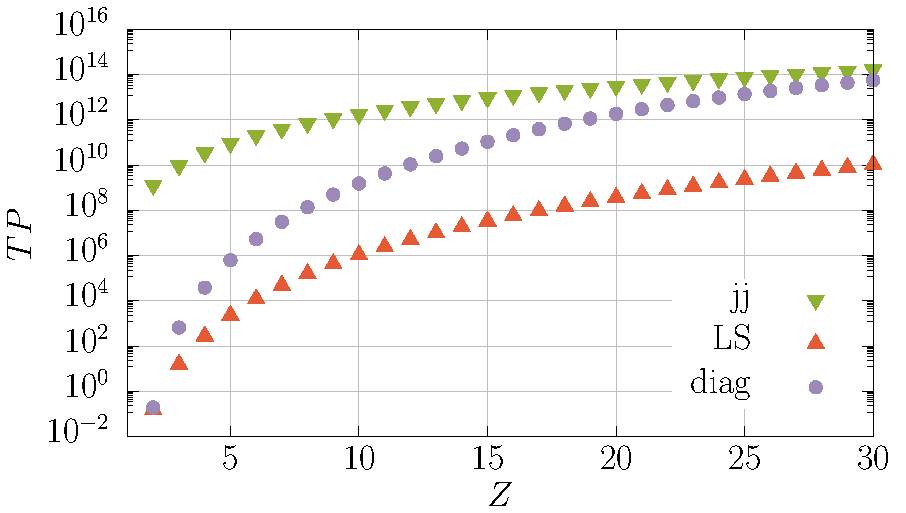
\includegraphics[width=130mm]{Graphs/LSvsjj.pdf}
    \caption{The probabilities of the~$1s^2 \rightarrow (1s 2p) {}^3P_1$ and~$1s^2 \rightarrow (1s_{1/2} 2p_{3/2})_1$ transitions are compared to the corresponding transition with exact coupling. It can be readily seen that~$LS$-coupling is accurate for small~$Z$, while~$jj$-coupling becomes more accurate as the nuclear charge increases. All data calculated with leading-order D-ECM.}
    \label{LSjjPlot}
\end{figure}

\section{Energies of excited states}
\label{sec:Coupling}

There remains one more question to be discussed - how to efficiently calculate excited energies. Excited states of atoms and ions tend to have much more degeneracy than the ground state and so one needs to be particularly careful about the definition of the specific zeroth-order electronic configurations. As mentioned in chapter~\ref{ch:secondECM}, in the case of multiple degenerate configurations, the multi-electron wavefunction can be obtained by diagonalizing the total Hamiltonian in the finite subspace spanned by the degenerate states. However since the number of possible configurations generally grows exponentially with the number of electrons, for the purpose of easy identification of states, approximate coupling schemes are often employed. In practice this means finding linear combinations of single-electron orbitals that result in definite values of the total quantum numbers of the multi-electron wavefunction.

\subsection{$LS$- vs.~$jj$-coupling}

The two simplest and most commonly used angular momentum coupling schemes are called~$LS$-coupling and~$jj$-coupling, referring to the specific quantum numbers that are fixed in the resulting configuration\footnote{By convention, small letters refer to quantum numbers of single-electron orbitals, while capital letters describe the total multi-electron wavefunction.}.

In the case of~$LS$-coupling the~$l$ and~$s$ quantum numbers of individual electrons add up to the total $L$ and $S$ of the multi-electron configuration respectively. For the purpose of evaluating relativistic corrections those can be further coupled to the total $J$ quantum number. For example, in the case of two-electron ions with one electron in the~$1s$ subshell and another in~$2p$, the possible~$LS-$coupled states are:
\begin{equation}
   (1s 2p) {}^1P_1,~~~~~~(1s 2p) {}^3P_1,~~~~~~(1s 2p) {}^3P_2.
\end{equation}

On the other hand, in the~$jj$-coupling scheme, the~$j$ quantum numbers of individual electrons add up to the total~$J$ quantum number of the multi-electron configuration. In the same example as above the three possible~$jj$-coupled states are:
\begin{equation}
   (1s_{1/2} 2p_{1/2})_1,~~~~~~(1s_{1/2} 2p_{3/2})_1,~~~~~~(1s_{1/2} 2p_{3/2})_2.
\end{equation}

\begin{figure}
    \centering
    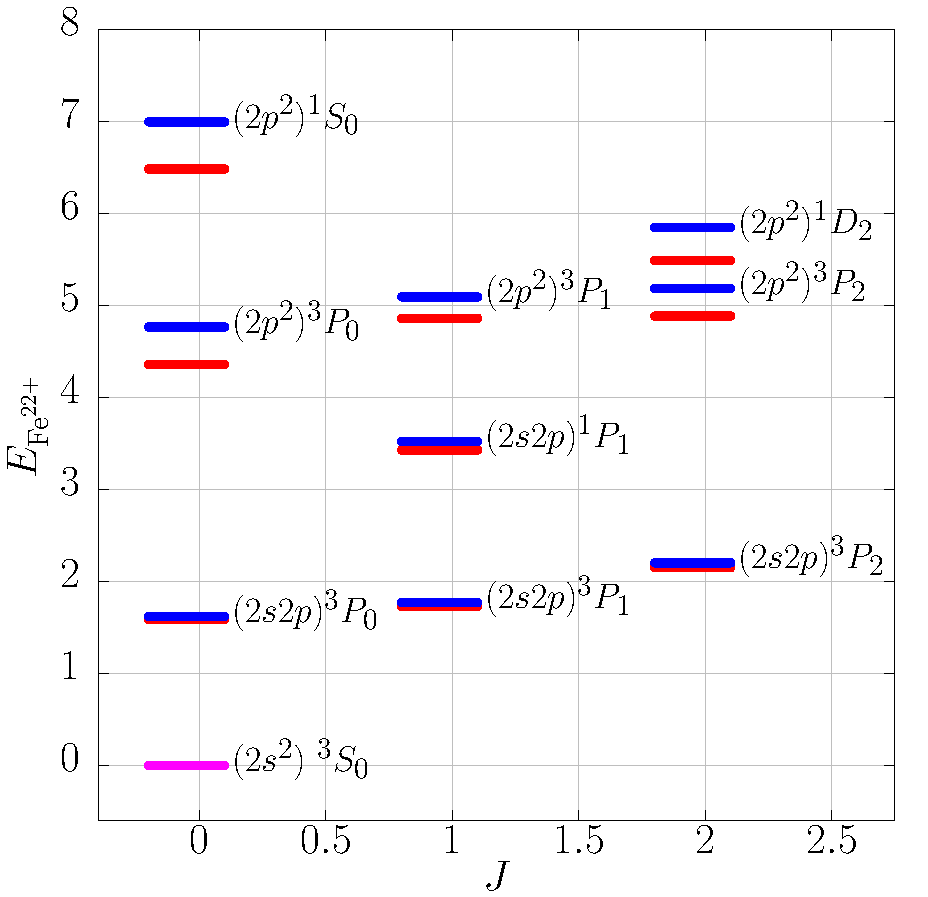
\includegraphics[width=69mm]{Graphs/ExcitedBerylium.pdf}
    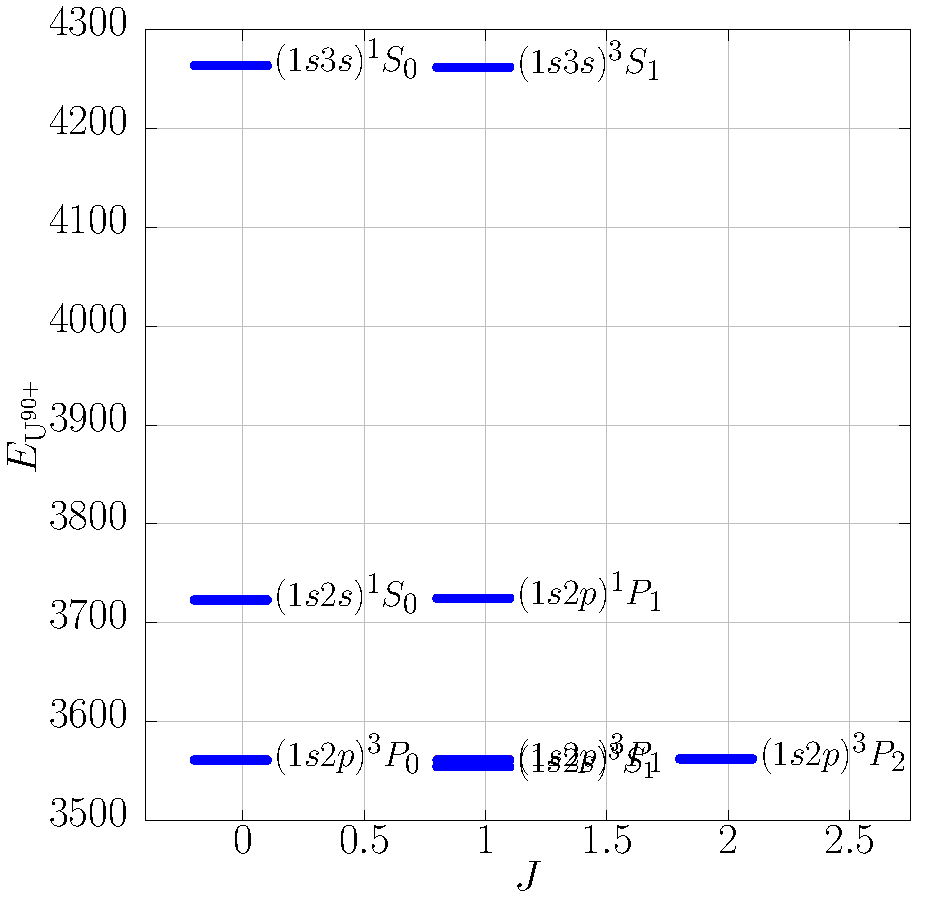
\includegraphics[width=69mm]{Graphs/ExcitedUlikeHe.pdf}
    \caption{Comparison of excited energies of~$_{26}$Fe${}^{22+}$ (left) and~${}_{92}$U${}^{90+}$ (right), calculated by diagonalizing a finite matrix in the leading-order ECM (blue) with references values (red). The reference values for~$_{26}$Fe${}^{22+}$ are taken from the NIST database~\cite{NIST} and for~${}_{92}$U${}^{90+}$ calculated with the  CI-DFS method~\cite{Tup2003OS}. The scale is fixed so that the energy of the ground state (pink) is equal to zero. Horizontal axis corresponds to total angular momentum quantum number of the multi-electron wavefunction. Numerical values given in Appendix~\ref{app:HCI}.}
    \label{ExcitedPlot}
\end{figure}


It is not always readily seen whether the~$LS$- and~$jj$-coupling scheme describe the same configurations. In this specific example only the third state is the same. The other two are related by the so-called~$LS$-$jj$ recoupling, which in this example happens to be
\begin{equation}
    \left(\begin{matrix}
    (1s 2p) {}^1P_1 \\
    (1s 2p) {}^3P_1
    \end{matrix}\right)
    =
    \frac{1}{\sqrt{3}}
    \left(\begin{matrix}
    \sqrt{2} & 1 \\
    1 & -\sqrt{2}
    \end{matrix}\right)
   \left(\begin{matrix}
    (1s_{1/2} 2p_{1/2})_1 \\
    (1s_{1/2} 2p_{3/2})_1
    \end{matrix}\right).
\end{equation}
In general, the $LS$-$jj$ recoupling is given by
\begin{equation}
    R_{LS \rightarrow jj} = \sqrt{(2L+1)(2S+1)(2j_1+1)(2j_2+1)}\left\{\begin{matrix}l_1&l_2&L\\s_1&s_2&S\\j_1&j_2&J\end{matrix}\right\},
\end{equation}
with the~$9j-$symbol defined in~\cite{9j}.

\subsection{State mixing}

It is important to emphasize that both of the above coupling schemes are approximations and the exact coupling can always be obtained by diagonalizing the Hamiltonian in the corresponding subspace. However, the resulting coefficients of the linear combination of single-electron orbitals, the so-called state mixing, depends on the nuclear charge~$Z$ and in the case of the ECM also influences the effective charge~$Z^*$. In practice, the~$LS$-coupling gives accurate predictions for low-$Z$ ions, while the~$jj$-coupling becomes more accurate as the nuclear charge increases. The transition cross-section calculation can be an interesting way of demonstrating that. As an example, in figure~\ref{LSjjPlot} the probabilities of the~$1s^2 \rightarrow (1s 2p) {}^3P_1$ and~$1s^2 \rightarrow (1s_{1/2} 2p_{3/2})_1$ transitions are compared to the corresponding transition with exact coupling for different values of~$Z$. It can be seen that the correct physical state, obtained from subspace diagonalization, corresponds to the~$LS$-coupled state only for~$Z \sim 2$, and then gradually gets closer to the~$jj$-coupled state as~$Z$ increases.

Despite the fact that the subspace diagonalization procedure is only necessary for degenerate states, it can also be useful in accounting for the mixing between states with small energy separation, that are nevertheless not strictly degenerate. This is because the perturbative corrections that these states contribute to each others values of energy are correspondingly larger. Since the subspace diagonalization procedure effectively accounts for all orders of perturbation coming from these states, it can describe low laying excited states of multi-electron atoms with good accuracy already in the leading-order. In figure~\ref{ExcitedPlot} we show the result of diagonalizing the~$1s^2 \{2s,2p,3s,3p\}^2$ subspace for be-like iron and the~$1s\{2s,2p,3s\}$ subspace for he-like uranium. Despite using  very small subspaces, both examples result in correct ordering of excited states already in the leading order, including all fine-structure states. 

